\documentclass[11pt]{beamer}

% ---------------------------------------------------------------------
% Preamble
% ---------------------------------------------------------------------

% ---------------------------------------------------------------------
% Packages
% ---------------------------------------------------------------------

\usepackage[utf8]{inputenc}
\usepackage{amsmath}
\usepackage{amssymb}
\usepackage[ngerman]{babel}
\usepackage{beamerprosper}
\usepackage{color}
\usepackage{epsfig}
\usepackage{graphicx}
\usepackage{epsfig}
\usepackage{latexsym}
\usepackage{listings}
\usepackage{times}
\usepackage{url}
\usepackage{xspace}
\usepackage{pgfpages}

% ---------------------------------------------------------------------
% Spacings
% ---------------------------------------------------------------------

\setlength{\parskip}{0.5ex}

% ---------------------------------------------------------------------
% Settings
% ---------------------------------------------------------------------

\lstset{ %
  backgroundcolor=\color{white},   % choose the background color; you must add \usepackage{color} or \usepackage{xcolor}
  basicstyle=\footnotesize\ttfamily, % the size of the fonts that are used for the code
  breakatwhitespace=false,         % sets if automatic breaks should only happen at whitespace
  breaklines=true,                 % sets automatic line breaking
  captionpos=b,                    % sets the caption-position to bottom
  commentstyle=\color{green},  	   % comment style
  deletekeywords={...},            % if you want to delete keywords from the given language
  escapeinside={\%*}{*)},          % if you want to add LaTeX within your code
  extendedchars=true,              % lets you use non-ASCII characters; for 8-bits encodings only, does not work with UTF-8
  frame=single,                    % adds a frame around the code
  keepspaces=true,                 % keeps spaces in text, useful for keeping indentation of code (possibly needs columns=flexible)
  keywordstyle=\color{blue},       % keyword style
  language=Java,                   % the language of the code
  morekeywords={*,...},            % if you want to add more keywords to the set
  numbers=left,                    % where to put the line-numbers; possible values are (none, left, right)
  numbersep=5pt,                   % how far the line-numbers are from the code
  numberstyle=\tiny\color{green},  % the style that is used for the line-numbers
  rulecolor=\color{black},         % if not set, the frame-color may be changed on line-breaks within not-black text (e.g. comments (green here))
  showspaces=false,                % show spaces everywhere adding particular underscores; it overrides 'showstringspaces'
  showstringspaces=false,          % underline spaces within strings only
  showtabs=true,                   % show tabs within strings adding particular underscores
  stepnumber=1,                    % the step between two line-numbers. If it's 1, each line will be numbered
  stringstyle=\color{blue},        % string literal style
  tabsize=2,                       % sets default tabsize to 2 spaces
  title=\lstname                   % show the filename of files included with \lstinputlisting; also try caption instead of title
}

% ---------------------------------------------------------------------
% Paths
% ---------------------------------------------------------------------

\graphicspath{{./images/}}

% ---------------------------------------------------------------------
% Theme
% ---------------------------------------------------------------------

\mode<all>
\usetheme{CambridgeUS}
\mode<presentation>
{
  \useinnertheme{rectangles}
  %\useoutertheme{}
  \setbeamercovered{transparent}
  \setbeamertemplate{navigation symbols}{}
}

% \definecolor{darkred}{rgb}{0.625,0.125,0.25}
\definecolor{darkred}{rgb}{0,0.4196,0.5803}
% \definecolor{bauhausblue}{rgb}{0,0.107,0.148}

\setbeamercolor{block body}{bg=gray!20}
\setbeamercolor{block title}{bg=darkred,fg=white}
\setbeamercolor{footlinecolorl}{fg=black,bg=lightgray}
\setbeamercolor{footlinecolor}{fg=black,bg=gray}
\setbeamercolor{footlinecolord}{fg=black,bg=darkgray}

\setbeameroption{show notes}
\setbeameroption{show notes on second screen=right}

% Auskommentieren, für Section 1,2,3, ...
\setbeamertemplate{section page}
{
    \begin{centering}
    \begin{beamercolorbox}[sep=12pt,center]{part title}
    \usebeamerfont{section title}\insertsection\par
    \end{beamercolorbox}
    \end{centering}
}

\setbeamertemplate{footline}{%
	\hbox{%
	\begin{beamercolorbox}[wd=.40\paperwidth,ht=4.25ex,left,leftskip=3ex]{author in head/foot}%
	    \vbox to4.25ex{\vfil\hbox{\usebeamerfont{author in head/foot} \insertshortauthor}\vfil}%
	\end{beamercolorbox}%
	\begin{beamercolorbox}[wd=.30\paperwidth,ht=4.25ex,center]{title in head/foot}%
	    \vbox to4.25ex{\vfil\hbox{\usebeamerfont{date in head/foot}\insertshorttitle{}}\vfil}%
	\end{beamercolorbox}%
  % \begin{frame number}{}
  % \end{frame number}%
	\begin{beamercolorbox}[wd=.30\paperwidth,ht=4.25ex,right,rightskip=3ex]{date in head/foot}%
	    % \vbox to4.25ex{\vfil\hbox{\insertshortdate{}}\vfil}%
      % \vbox to4.25ex{\vfill\hbox{frame number}}
      \vbox to4.25ex{\vfill\hbox{\insertframenumber{} / \inserttotalframenumber }\vfill}
	\end{beamercolorbox}}%
}
%\setbeamertemplate{footline}{
%  \quad \tiny \insertshortauthor \hfill \insertshorttitle \qquad \hfill \insertshortdate\ \qquad\qquad
%}
\setbeamertemplate{theorems}[numbered]
% ---------------------------------------------------------------------
% Commands
% ---------------------------------------------------------------------

\newcommand{\eg}{\textit{e.g.,}\xspace}
\newcommand{\shortsep}{||}
\newcommand{\sep}{\ \shortsep \ }
\def\getpdfpages#1#2{\begingroup
  \setbeamercolor{background canvas}{bg=}
  \includepdf[pages={#1},%
  pagecommand={\global\setcounter{framenumber}{\value{page}}%
    \expandafter\def\expandafter\insertshorttitle\expandafter{%
      \insertshorttitle\hfill\insertframenumber\,/\,\inserttotalframenumber}}%
  ]{#2}
  \endgroup}

% ---------------------------------------------------------------------
% Title
% ---------------------------------------------------------------------

\title[Bauhausboards]{Bauhausboards\\Interactive Door Signs for the Office}
\subtitle{Bachelorverteidigung}
\author[André Karge]{André Karge}
\institute[Bauhaus-Universität Weimar]{
\includegraphics[width=0.5\textwidth]{buw-logo}}
\date[29.02.2016]{29.02.2016}

\raggedright
\AtBeginSection{\frame{\sectionpage}}

% ---------------------------------------------------------------------

\begin{document}

% ---------------------------------------------------------------------
% Content
% ---------------------------------------------------------------------

\maketitle

\begin{frame}{Agenda}
\tableofcontents
\end{frame}
% ---------------------------------------------------------------------
\section{Grundlagen}
% - Einführung in Interaktive Türschilder
% - Netboards als Vorlageprojekt
%   * ein wenig Netboards erklären
% - Entscheidungspunkt: Eigenes System "Bauhausboards" entwickeln
\begin{frame}{Türschilder}
  Nutzung von Türschildern in Forschungseinrichtungen
  \note<1>{
    Türschilder in Forschungseinrichtungen als Informationsschnittstelle zwischen Arbeiter in Büro - Gästen oder Kollegen\\
    Das sind:\\
    \begin{itemize}
      \item Whiteboards
      \item Tafeln
      \item Post-It Zettel
      \item Bitte-Nicht-Stören-Schilder
    \end{itemize}
  }
  \pause
  \begin{itemize}
    \item Darbietung persönlicher Informationen
    \note<2>{
      Dienen zu:
      \begin{itemize}
        \item Darbietung persönlicher Daten (sind Informationen aller Art)
        \begin{itemize}
          \item Handskizzen
          \item Texte
          \item Ausdrucke
          \item Statusmeldungen (bspw.: bin gleich wieder da / die ganze Woche auf Forschungsreise)
        \end{itemize}
      \end{itemize}
    }
    % \pause
    \item Kommunikation zwischen Mitarbeitern und Gästen
    \note<2>{
      \begin{itemize}
        \item Kommunikation zwischen Mitarbeitern / Gästen
        \begin{itemize}
          \item an was arbeiten die Kollegen / Arbeiter in den Büros
          \item das heißt: Forschungsarbeit oder lustiger Inhalt
        \end{itemize}
      \end{itemize}
    }
  \end{itemize}
    % - Darbietung von persönlichen Daten (Informationen aller Art - Handskizzen, Texte, Ausdrucke, Statusmeldungen(bin gleich wieder da))
    % - Kommunikation zwischen Mitarbeitern / Gästen
\end{frame}

\begin{frame}
  % \todo{hier ein Bild von einem Whiteboard in der B11}
  \begin{center}
    aktuelle Situation?\\~\\
    \pause
    \visible<2>{
      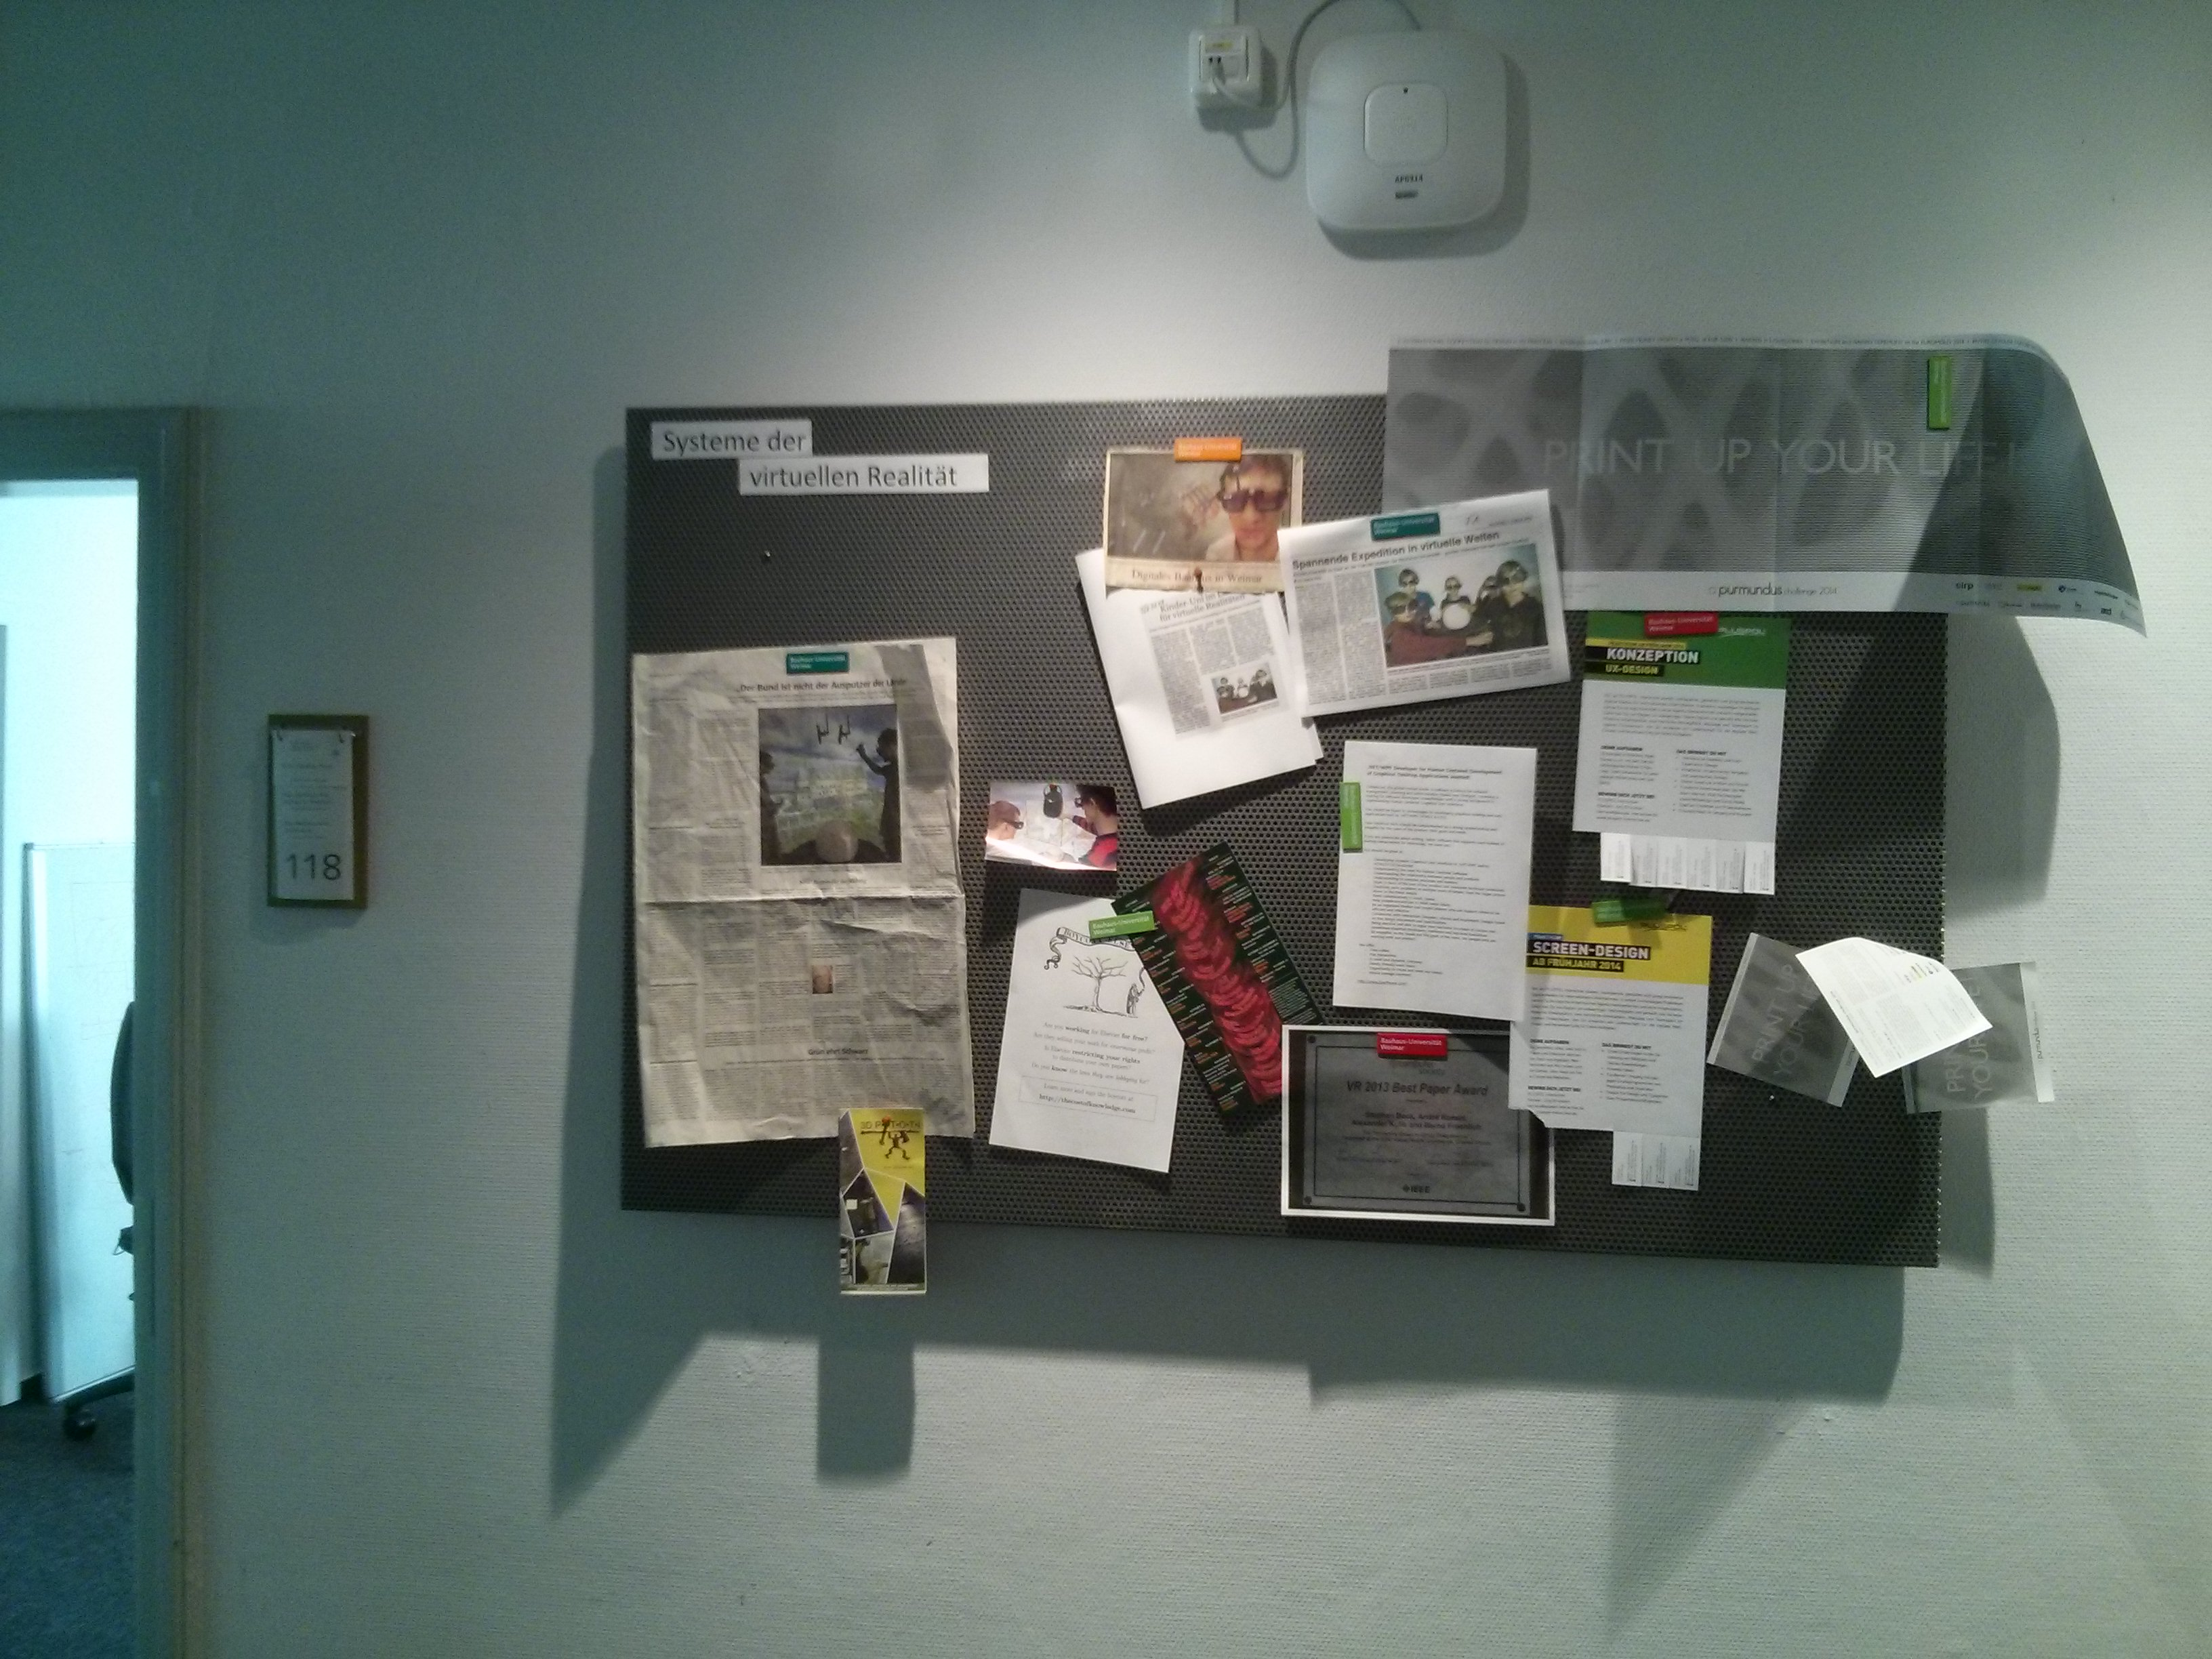
\includegraphics[width=0.7\textwidth]{pinnwand}
    }
  \end{center}
  \note<1-2>{
    Aber: Wie sieht das aktuell aus? -click-\\
    Aushänge erzeugen periphere Aufmerksamkeit\\
    \todo{bild schöner machen}
  }
\end{frame}

\begin{frame}{Nachteile}
  \note<1>{
    Aus analoger Form der Informationsdarbietung: Nachteile\\
  }
  Nachteile von analogen Türschildern:
  \pause
  \begin{itemize}
    \item Man muss persönlich vor Ort sein
    \pause
    \item ungewünschtes Entfernen / Hinzufügen / Ändern von Information durch Dritte
  \end{itemize}
  \note<2>{
    Vor Ort sein:
    \begin{itemize}
      \item Änderung des eigenen Inhaltes nur, wenn man persönlich vor Ort ist
      \item Oder: man jemand anderes, der vor Ort ist mit Änderung beauftragt
      \item selbes auch bei hinterlassenen Nachrichten
    \end{itemize}
  }
  \note<3>{
    Vandalismus:
    \begin{itemize}
      \item jeder Vorbeigehende kann nach Belieben Texte/Bilder ändern/hinzufügen/entfernen
      \item $\rightarrow$ Möglichkeit von Vandalismus sehr hoch
    \end{itemize}
  }
    % - Content kann nur geändert werden, wenn man persönlich vor Ort ist
    % - Hinterlassene Nachrichten können nur gelesen werden, wenn man selbst vor Ort ist
    % - Zudem können Gäste den bestimmte Sachen abwischen / neue hinzufügen (Vandalismus)
\end{frame}
\begin{frame}{Lösung}
  \note<1>{
    Eine Lösung ist das Anbringen von interaktiven digitalen Türschildern
  }
  \begin{itemize}
    \item Anbringung von digitalen Türschildern
    \pause
    \begin{itemize}
      \item Änderung von präsentierten Inhalten aus der Ferne
      \item Erhalten von Mitteilungen ohne vor Ort zu sein
      \item Einschränkung von Vandalismus
    \end{itemize}
  \end{itemize}
  \note<2>{
    \begin{itemize}
      \item Vorteil: man muss nicht mehr selbst vor Ort sein um Inhalt zu ändern / Nachrichten zu erhalten
      \item Durch Eingrenzung der Interaktionsmöglichkeiten: Einschränkung von Vandalismus (Nutzungsrechte)
    \end{itemize}
  }
    % - Interaktive Türschilder
    % - Digitaler Ersatz für Whiteboards/Tafeln neben Büros
    % - Nutzer müssen nicht mehr persönlich vor Ort sein, um Content zu ändern / Nachrichten zu empfangen
    % - Vandalismus wird eingeschränkt
\end{frame}

\begin{frame}[t]{Vorarbeit}
  \note<1-3>{
    Dazu: einige Projekte mit ähnlichem Ansatz:
    \begin{itemize}
      \item Hermes (2003) Universität Lancaster (etwas älteres Projekt)
      \item NetBoards (2014) Universität Cambridge (aktuelleres Projekt)
    \end{itemize}
    NetBoards am Anfang der Arbeit in einer Vorstudie aufgesetzt.\\
    Ergebnis $\rightarrow$ eigenes Projekt\\
    (da Interaktion zu offen und Vandalismusmöglichkeit zu hoch)
  }
  \pause
  \begin{columns}[t]
    \begin{column}{0.49\textwidth}
      \begin{center}
        \visible<2-3>{
          Hermes (2003)\\
          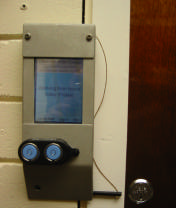
\includegraphics[width=0.7\textwidth]{hermes_display}\\
          \quelle{Quelle: Keith Cheverest et. al. - Ambient Intelligence 2003}
        }
      \end{center}
    \end{column}
    \pause
    \visible<3>{
      \begin{column}{0.49\textwidth}
        \begin{center}
          NetBoards (2014)\\
          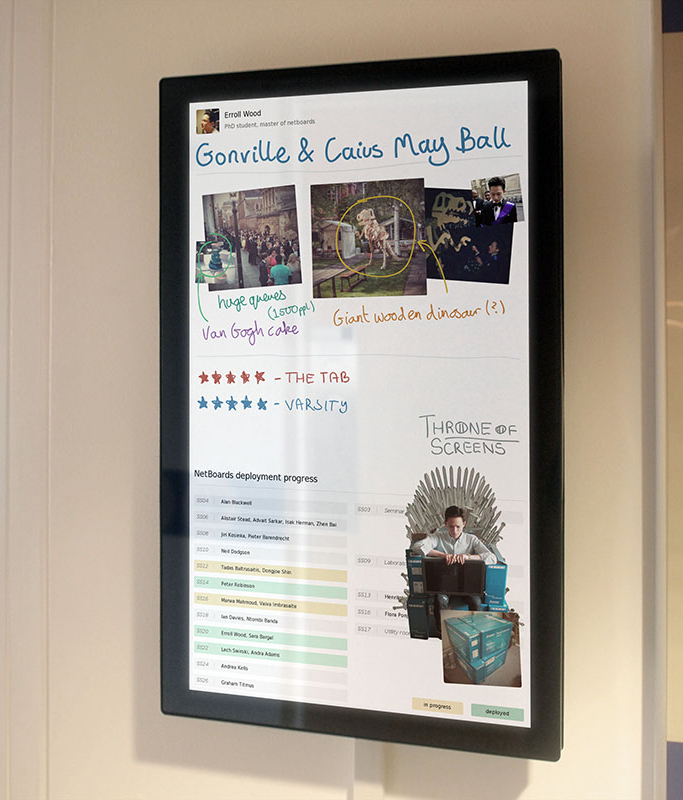
\includegraphics[width=0.705\textwidth]{netboards}\\
          \quelle{Quelle: Errol Wood et. al. - ACM ITS 2014}\\
        \end{center}
      \end{column}
    }
  \end{columns}
  % \pause
  % NetBoards in kleiner Studie aufgesetzt\\
  % Als Ergebnis: eigenes Projekt

  %   - Hermes (2003)
  %   - Netboards (2014)
  % - Ergebnis aus Vorstudie mit NetBoards: eigenes Projekt
\end{frame}

  % - Türschilder
  %   - Darbietung von persönlichen Daten (Informationen aller Art - Handskizzen, Texte, Ausdrucke, Statusmeldungen(bin gleich wieder da))
  %   - Kommunikation zwischen Mitarbeitern / Gästen
  % - Problem?:
  %   - Content kann nur geändert werden, wenn man persönlich vor Ort ist
  %   - Zudem können Gäste den bestimmte Sachen abwischen / neue hinzufügen (Vandalismus)
  %   - Hinterlassene Nachrichten können nur gelesen werden, wenn man selbst vor Ort ist
  % - Lösung:
  %   - Interaktive Türschilder
  %   - Digitaler Ersatz für Whiteboards/Tafeln neben Büros
  %   - Nutzer müssen nicht mehr persönlich vor Ort sein, um Content zu ändern / Nachrichten zu empfangen
  %   - Vandalismus wird eingeschränkt

  % - Andere Projekte mit selbem Ansatz
  %   - Hermes (2003)
  %   - Netboards (2014)

  % - Ergebnis aus Vorstudie mit NetBoards: eigenes Projekt

  % wie lange dauert der Abschnitt?? max 10min!!
% \end{frame}
% ---------------------------------------------------------------------
\section{Umsetzung}
% - Bauhausboards
%   * Webapplikation mit Webserver
%   * NodeJS Serverseitig
%   * HTML+CSS+Javascript Clientseitig
%   * Wichtigste Komponente: Editor mit Paper.js
%   * User Frontend + User Backend
%   * wichtigste Funktionen:
%     # User-Content
%     # Messageing System
%     # (beides auf Editor-Grundlage)
%     # Remote-Änderung des Contents
%     # Remote-Einsicht von Messages da per Mail
\begin{frame}{Bauhausboards}
  \pause
  \begin{center}
    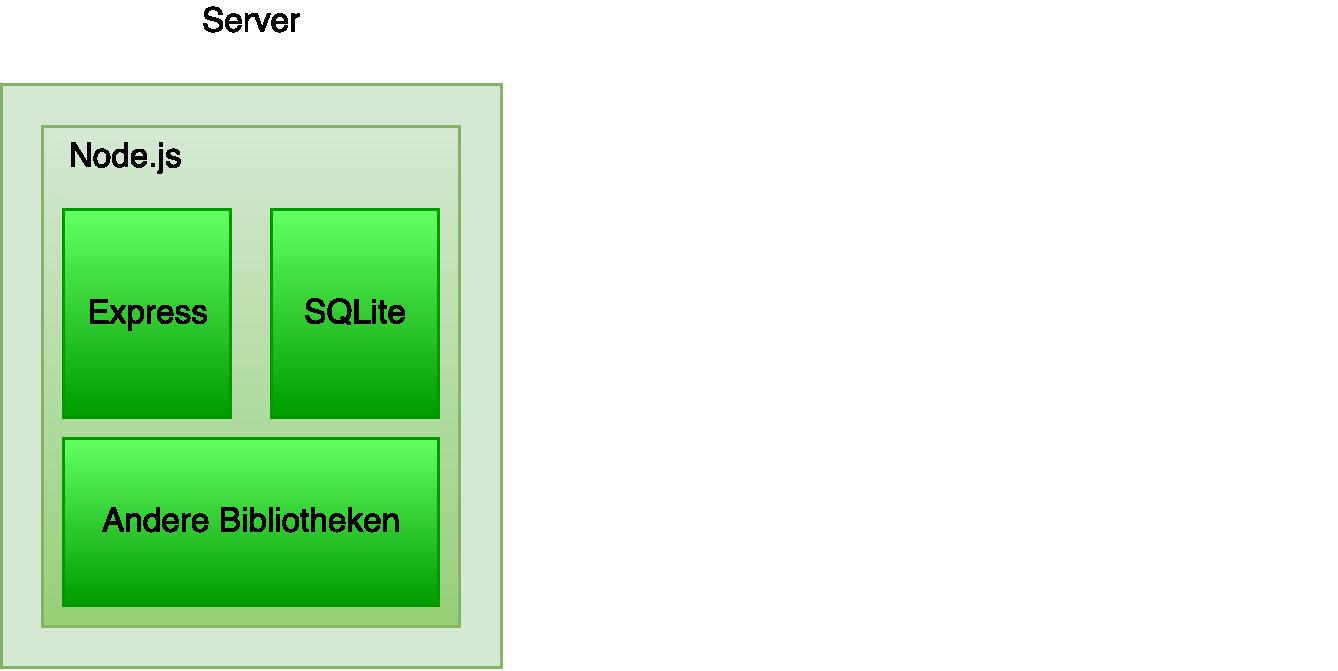
\includegraphics[width=0.9\textwidth]{presBaBo-1.pdf}
  \end{center}
  \note<1>{
    \begin{itemize}
      \item andere Möglichkeiten: Tablet-App (Android, iOS, Windows-Mobile)
      \item Problem: Erhöhter Aufwand durch Portierung
      \item Deswegen: Entscheidung: Entwurf von Web-Applikation
      \item System besteht aus: -click-
    \end{itemize}
  }
  \note<2>{
    \begin{itemize}
      \item einfacher Webserver (NodeJS Serversprache)
      \item besteht aus mehreren Bibliotheken
      \begin{itemize}
        \item Express = Framework zum Erstellen des Grundgerüsts einer Webseite
        \item SQLite = Datenbank-Bibliothek
        \item mehreren anderen Bibliotheken (Email.js, Crypto.js, twitter.js)
      \end{itemize}
    \end{itemize}
  }
\end{frame}
\begin{frame}[noframenumbering]{Bauhausboards}
  \begin{center}
    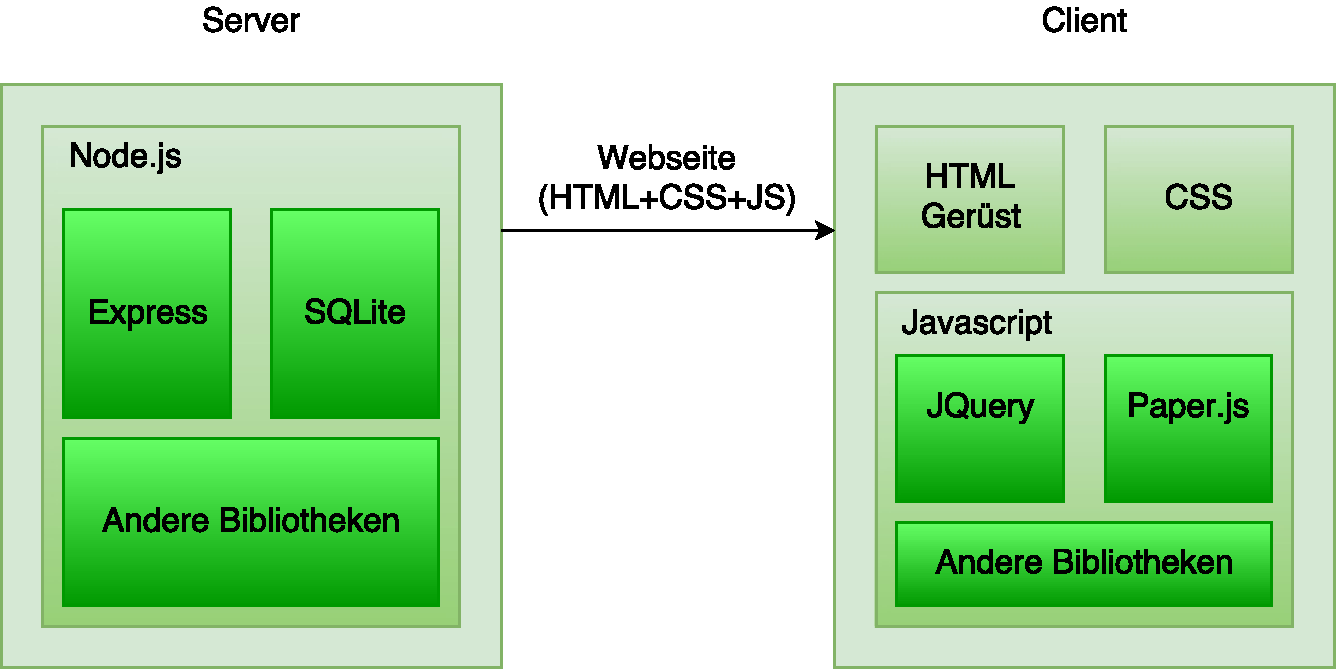
\includegraphics[width=0.9\textwidth]{presBaBo-2.pdf}
  \end{center}
  \note<1>{
    \begin{itemize}
      \item Webserver liefert Webseite an Clients aus
      \item Webseite besteht aus dem Express-Grundgerüst + CSS + allen Javascript Funktionen
      \item Javascript-Funktionalität hauptsächlich:
      \begin{itemize}
        \item JQuery zur Manipulation des Seitenaufbaus+Datenaustausch mit Server -click-
        % \item Paper.js als Vector-Grafik-Framework (Editor basiert darauf)
        % \item andere kleinere Bibliotheken
      \end{itemize}
    \end{itemize}
  }
\end{frame}
\begin{frame}[noframenumbering]{Bauhausboards}
  \begin{center}
    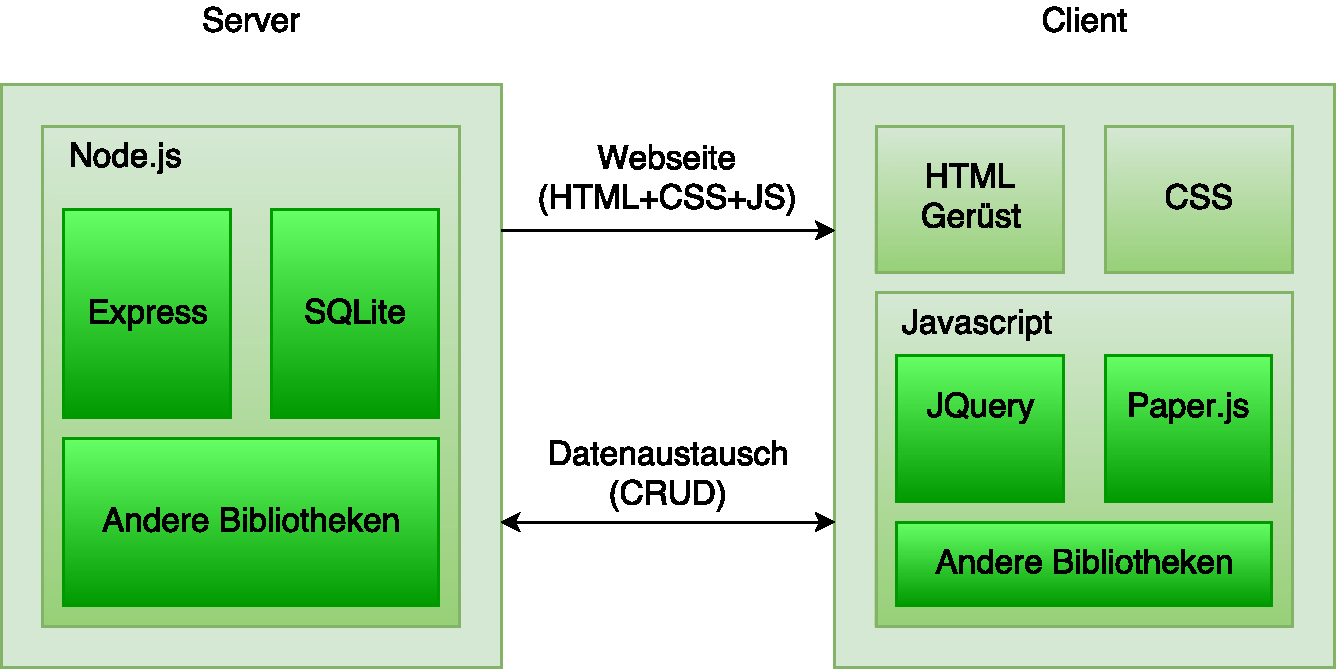
\includegraphics[width=0.9\textwidth]{presBaBo-3.pdf}
  \end{center}
  \note<1>{
    \begin{itemize}
      \item \textcolor{gray}{JQuery zur Manipulation des Seitenaufbaus+Datenaustausch mit Server -click-}
      \item Paper.js als Vector-Grafik-Framework (Editor basiert darauf)
      \item andere kleinere Bibliotheken
      \item Datenaustausch mit Server über CRUD-Prinzip\\(C(create) R(ead) U(pdate) D(elete))
    \end{itemize}
  }
\end{frame}

\begin{frame}{Editor}
  % Funktionen:
  % \begin{itemize}
  %   \item Zeichnen mit Stiften
  %   \item Anheftung von Bildern
  %   \item Entfernung von Elementen
  %   \item Neuanordnung angehefteter Elemente
  % \end{itemize}
  Funktionen:\\
  \todo{color here}
  \pause
  \begin{columns}[t]
  % \hline
  % \vrule{}
    \begin{column}{0.24\textwidth}
      \begin{center}
        \textbf{Zeichnen}\\mit\\verschieden-\\farbigen Stiften
      \end{center}
    \end{column}
    % \vrule{}
    \pause
    \begin{column}{0.24\textwidth}
      \begin{center}
        \textbf{Anheften}\\von\\Bildern und Zetteln
      \end{center}
    \end{column}
    % \vrule{}
    \pause
    \begin{column}{0.24\textwidth}
      \begin{center}
        \textbf{Neuanordnen}\\von\\Bildern und Zetteln
      \end{center}
    \end{column}
    % \vrule{}
    \pause
    \begin{column}{0.24\textwidth}
      \begin{center}
        \textbf{Entfernen}\\von\\Zeichnungen, Bildern und Zetteln
      \end{center}
    \end{column}
    % \vrule{}
    % \hline
  \end{columns}

  % \todo{Step by Step Icons - Stift,Schwamm,Pinnnadel,Hand}

  \note<1-5>{
    \begin{itemize}
      \item Hauptkomponente von Bauhausboards = Editor
      \item sollte annähernd Funktionen von Tafel/Whiteboard haben -click-
      \begin{itemize}
        \item Zeichnen mit verschiedenfarbigen Stiften (unterschiedlicher Dicke)
        \item Anheften von Bildern/Zetteln (per Magnet oder Pinnadel)
        \item Entfernen von gezeichneten Elementen (Schwammfunktion / Zettel entfernen)
        \item Neuanordnung angehefteter Elemente
      \end{itemize}
    \end{itemize}
  }
\end{frame}
\begin{frame}{Editor}
  % \pause
  \todo{folie fertig machen}\\
  \todo{Bilder vom Editor}\\
  \note<1>{
    \begin{itemize}
      \item realisiert mit dem Javascript-Framework Paper.js
      \item Nutzerinhalt(auf Basis von Editor)
      \item Nachrichtensystem(auf Basis von Editor)
    \end{itemize}
  }
\end{frame}
\begin{frame}{Vorteile}
  \begin{itemize}
    \item Von Überall erreichbar
    \pause
    \item Erhöhte Sicherheit vor Vandalismus
    \pause
    \item Darstellung von animiertem Inhalt
  \end{itemize}
  \note<1-3>{
    \begin{itemize}
      \item Da man von Überall auf den Server zugreifen kann: nicht notwendig direkt vor Ort zu sein
      \item Sicherheitsaspekt, da nur angemeldete Nutzer präsentierten Inhalt ändern können
      \item Präsentation von Animierten Inhalten (zur Zeit nur Gifs)
      \item (System musste auf Nutzbarkeit getestet werden)
    \end{itemize}
  }
\end{frame}

  % - Bauhausboards
  % - Web-Applikation
  %   - Serverseitig
  %     - NodeJS für Serversprache
  %     - SQLite für Datenbank
  %   - Clientseite
  %     - HTML+CSS Webseite ausgeliefert
  %     - Javascript mit JQuery für HTML-DOM Manipulation und Funktionalitäten
  %   - Kommunikation Client-Server
  %     - erster Aufruf liefert Webseite und Funktionalitäten (JS) aus
  %     - Dynamisches Nachladen von Daten per Ajax (CRUD Prinzip)
  %   - Komponenten
  %     - Editor - Da Simulation von Tafel/Whiteboard
  %       - Editorfunktionen
  %         - Zeichnen mit verschiedenfarbigen Stiften
  %         - Schwammfunktion zum Entfernen von gezeichneten/geschriebenen Elementen
  %         - Anheften von Bildern/Zetteln per bspw.: Magneten
  %         - Neuanordnung von angehefteten Elementen
  %       - realisiert mit dem Javascript-Framework Paper.js
  %     - Nutzerinhalt(auf Basis von Editor)
  %     - Nachrichtensystem(auf Basis von Editor)
  %   - Vorteile gegenüber Whiteboards/Tafeln:
  %     - Da man von Überall auf den Server zugreifen kann: nicht notwendig direkt vor Ort zu sein
  %     - Sicherheitsaspekt, da nur angemeldete Nutzer präsentierten Inhalt ändern können
  %     - Präsentation von Animierten Inhalten (zur Zeit nur Gifs)
  % - Überleitung zur Studie
  %   - Das System musste auf Nutzbarkeit getestet werden
% \end{frame}
% ---------------------------------------------------------------------
\section{Studie}
% - Studie
%   * System musste getestet werden
%   * 9 Tester á 4 Räume via 4 Tablets
%   * Tutorial mit allen Funktionen erstellt
%   * 2 Wochen Laufzeit
%   * Auswertung der Studie
%     # Interview zum Sammeln von Feedback (Anzahl von Fragen mit angeben vllt noch Beispielfragen)
%     # UEQ Fragebogen
\begin{frame}{Testsystem}
  \note<1>{
  - Testsystem aufgesetzt\\
    - Webserver\\
    - 4 Tablets mit Webprowser im Kiosk-Modus\\
  - How-To-Pdf aufgestzt, mit allen Funktionen des System und wie sie zu benutzen sind\\
  - Tablets vor Büros in der Bauhausstraße 11 angebracht\\
  - Studienlaufzeit: 2 Wochen\\
    - dabei:\\
      - Nutzer erzeugten diverse Inhalte(meistens Fun aber auch informativ)\\
      - Gäste hinterließen Nutzern Nachrichten (dabei aber auch ab und an ohne Kontext/ temporäres Graffiti)\\
  }
\end{frame}
\begin{frame}{Auswertung}
  \note<1>{
  - Auswertung der Studie durch Interviews + Fragebogen\\
    - 5h 30min an Interview-Mitschnitten zur besseren Analyse\\
    - Fragenkatalog mit Fragen zu bestimmten Systemfunktionen\\
    - UEQ (User-Experience-Questionaire) als Standardevaluationsmethode\\
  }
\end{frame}
\begin{frame}{Studienergebnisse}
  \note<1>{
    - wurde größtenteils wegen der Möglichkeit bewegten Inhalt zu erstellen genutzt (das heißt viele Gifs usw.)\\
    - 2 Eingebaute Authentisierungsmethoden waren hinderlich\\
    - einigen Nutzern waren manche Schritte zu kompliziert\\
    - Authorenkennzeichnung in Nachrichten hat gefehlt (größtes Manko)\\
    - Emails bekommen durch Skizzen eine persönliche Note\\
  }
\end{frame}
%   - Testsystem aufgesetzt
%     - Webserver
%     - 4 Tablets mit Webprowser im Kiosk-Modus
%   - How-To-Pdf aufgestzt, mit allen Funktionen des System und wie sie zu benutzen sind
%   - Tablets vor Büros in der Bauhausstraße 11 angebracht
%   - Studienlaufzeit: 2 Wochen
%     - dabei:
%       - Nutzer erzeugten diverse Inhalte(meistens Fun aber auch informativ)
%       - Gäste hinterließen Nutzern Nachrichten (dabei aber auch ab und an ohne Kontext/ temporäres Graffiti)
%   - Auswertung der Studie durch Interviews + Fragebogen
%     - 5h 30min an Interview-Mitschnitten zur besseren Analyse
%     - Fragenkatalog mit Fragen zu bestimmten Systemfunktionen
%     - UEQ (User-Experience-Questionaire) als Standardevaluationsmethode
%   - Ergebnisse der Studie
%     - wurde größtenteils wegen der Möglichkeit bewegten Inhalt zu erstellen genutzt (das heißt viele Gifs usw.)
%     - 2 Eingebaute Authentisierungsmethoden waren hinderlich
%     - einigen Nutzern waren manche Schritte zu kompliziert
%     - Authorenkennzeichnung in Nachrichten hat gefehlt (größtes Manko)
%     - Emails bekommen durch Skizzen eine persönliche Note
% \end{frame}
% ---------------------------------------------------------------------
\section{Ausblick}
% - Ausblick
%   * Strukturänderungen am System (Frontend - Backend Trennung) - als Konsequenz der Studie
%   * Poweruser Einstellung
%   * Audio-/Video-/Fotonachrichten
\begin{frame}{Ausblick}
  \note<1>{
  - Als Schlussfolgerung:\\
    - Änderungen am System müssen durchgeführt werden\\
      - Poweruserfunktion\\
      - Audio-/Video-/Fotonachrichten\\
      - Strukturänderungen - Trennung Frontend-Backend\\
    - erneute (längere+größere) Studie mit eingebauten Änderungen\\
  }
\end{frame}
% ---------------------------------------------------------------------
\section*{Demo}
% \begin{frame}
% - Demo
%   * Frontend Demo meiner Wall
%   * --> Jemand schreibt eine Nachricht --> Mail erhalten / Einsicht im User-Backend
%   * Änderung des Wallcontents
%   * Gifs + Twitter
  % \begin{center}
  %   Demo
  %   % \todo{vor oder nach Fragerunde?}
  % \end{center}
% \end{frame}
\section*{Fragen?}
% \begin{frame}
%   \begin{center}
%     Fragen?
%   \end{center}
% \end{frame}
\section*{Danke für ihre Aufmerksamkeit!}
% \begin{frame}
%   \begin{center}
%     Danke für ihre Aufmerksamkeit!
%   \end{center}
% \end{frame}


















% % ---------------------------------------------------------------------
% \section{Aufbau eines Vortrags}
% % ---------------------------------------------------------------------

% \begin{frame}{Aufbau eines Vortrags}
%   \begin{itemize}
%     \item Motivation des Themas
%     % \pause
%     \item Erläuterung der Problemstellung
%     % \pause
%     \item Bisherige/Mögliche Ansätze
%     \begin{itemize}
%         \item Ansatz 1
%         \item Ansatz 2
%     \end{itemize}
%     \item Eigene Lösung oder -versuche
%     \item Zusammenfassung oder Schlussfolgerung
%   \end{itemize}
% \end{frame}

% % ---------------------------------------------------------------------
% \section{Layouts}
% % ---------------------------------------------------------------------

% \begin{frame}{Block- und Mathe-Umgebungen}
% \begin{block}{Definition}
% Dies ist eine Definition.
% $$ a^2 + b^2 = c^2 $$
% \end{block}
% Der erste Buchstabe im griechischen Alphabet ist $\alpha$.
% Grafiken lassen sich einfach mit \texttt{\textbackslash includegraphics} einfügen.
% 
\includegraphics[width=0.7\textwidth]{buw-logo}
% \end{frame}

% % ---------------------------------------------------------------------

% \begin{frame}{Mehrspaltig}
%   Mit Hilfe von \texttt{\textbackslash columns} lassen sich mehrspaltige Folien erstellen.
%   \begin{columns}
%     \begin{column}{0.32\textwidth}
%         
\includegraphics[width=0.9\textwidth]{Tux}
%     \end{column}
%     \begin{column}{0.32\textwidth}
%         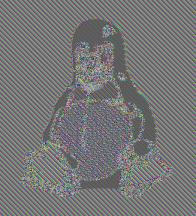
\includegraphics[width=0.9\textwidth]{Tux_ecb}
%     \end{column}
%     \begin{column}{0.32\textwidth}
%         
\includegraphics[width=0.9\textwidth]{Tux_secure}
%     \end{column}
%   \end{columns}
% \end{frame}

% % ---------------------------------------------------------------------

% \begin{frame}{Tabellen}
%   Tabellen sind auch ganz einfach.
%   \begin{table}
%     \begin{tabular}{lcr}
%         \hline
%         Linksbündig & Zentriert & Rechtsbündig \\
%         \hline
%         1 & 2 & 3 \\
%         4 & 5 & 6 \\
%         \hline
%     \end{tabular}
%     \caption{Tabellenunterschrift}
%   \end{table}
% \end{frame}

% % ---------------------------------------------------------------------

% \begin{frame}{Weitere Informationen}
%   Homepage: \\
%   \url{https://bitbucket.org/rivanvx/beamer/wiki/Home}
  
%   Benutzerhandbuch: \\
%   \url{http://www.ctan.org/tex-archive/macros/latex/contrib/beamer/doc/beameruserguide.pdf}
  
%   Wiki LaTeX-Kompendium: \\
%   \url{http://de.wikibooks.org/wiki/LaTeX-Kompendium}
  
%   Stack Exchange für LaTeX: \\
%   \url{http://tex.stackexchange.com/}
  
%   Symbolsuche: \\
%   \url{http://detexify.kirelabs.org/classify.html}
% \end{frame}

% % ---------------------------------------------------------------------

% \begin{frame}[fragile]{Listing}
% \begin{lstlisting}
% public class Calculator {

%     private int memory;

%     public int add(int a, int b) {
%         String foo = "bar"; // Just to demonstrate strings
%         return a + b;
%     }

%     /**
%      * Very important function!
%      * Good comments are essential to deliver high-quality code!
%      */
%     public int multiply(int a, int b) {
%         return a * b;
%     }
% }
% \end{lstlisting}
% \end{frame}

% % ---------------------------------------------------------------------
% % Appendix
% % ---------------------------------------------------------------------

% \appendix
\end{document}
